\chapter{Introduction}
\label{chap:01_introduction}

% \todo[inline]{
% Margins needs to be reduced back in layout.tex to
% "oddsidemargin 2.7cm", "evensidemargin 2.6cm"
% and "usepackage[paperwidth=275.9mm, paperheight=279.4mm]{geometry}"
% in Thesis.tex needs to be removed.}

% - why other theories do not fit into this problem (like finger printing, beam forming)
% -> TDOA between robots -> one does not want to send signal samples
%    via message. (Too large information)
%   -> Approach of Dortmund -> too inaccurate time point when whistle is detected. NTP too
%      inaccurate, offline synchronization can be done or PTP implementation
% Another approach would be the TDOA between the robots. Therefore, the robots needs to
% be synchronized in time. The whistle detection time point can then be taken for calculating
% the time difference of arrival. The distance between the robots needs to be known
% Robots needs to be synchronized (which is difficult with NTP only)

\acf{SSL} is content of research for many years with
application scenarios in various environments due to its
validity for all sorts of signals (sonar, radar, acoustic, seismology,
geophysics, ultrasonics, communications \cite{Chen2006}) 
Explicitly for audio signals, use cases emerge with the progressing
ordinariness of technical equipment on daily basis.
% As technical devices gained in importance more and more,
Assuming robots as forthcoming everyday object, reaction to acoustic
input is one essential step for natural human-robot interaction.
For example, one plausible scenario is a humanoid robot keeping the eye
contact with an interacting human.
An even more tangible case can be seen in conference rooms of business environments
where remote participation is commonplace in these days.
Functions of communication systems like speaker identification and tracking of active talkers
get crucially important to provide smooth operation \cite{Brandstein96apractical}.
In general, \ac{SSL} algorithms can be divided into three categories
which are based on beamforming, eigenvalue decomposition or \ac{TDOA} \cite{Brandstein96apractical}.
% intuitive handling with acoustic input
% Especially, many use cases exist regarding non-acoustic signals
% like sonar, radar,
% investigated by researchers a broad topic which is
% In this field of signal processing, signal source localization is

In this thesis, the \ac{TDOA} method was chosen to estimate the \ac{SSL} and evaluates
different implementations focussing on whistle sounds in the context of an engineering competition
\textit{\ac{RoboCup}}.
As \cite{BAS_estimator} states, beamforming is computationally expensive and eigenvalue
decomposition is little suitable
for signals with small bandwidth which is why the \ac{TDOA} method was selected as most
appropriate solution.
A widespread approach is to cross-correlate the sensor readings of two microphones
to obtain the time delay between those.
By this, the direction of a signal source can be derived by geometrical relation by one
stand-alone system and a position by a multi-agent system.

\section{Motivation}

The \acf{RoboCup} is known for promoting research on autonomous robotic systems
by scientists and students of universities.
It offers a platform, where focus is set on fast intelligent systems and multi-agent
collaboration \cite{robocup}.
This initiative encourages young engineers to work in real case scenarios
by providing several leagues with different engineering tasks that are required
on the subject of robotics.

In the \ac{SPL} of the \ac{RoboCup}, humanoid robots are developed to play soccer autonomously
for scientific purpose.
By requirement, the hardware is identical for all competitors in this league and no modification
is allowed.
Since 2008 commercially available humanoid robots named \textit{NAO} provided by the
company \textit{SoftBank Robotics} are used.
% -------------------------------------------------------------
\begin{figure}[ht]
	\centering
        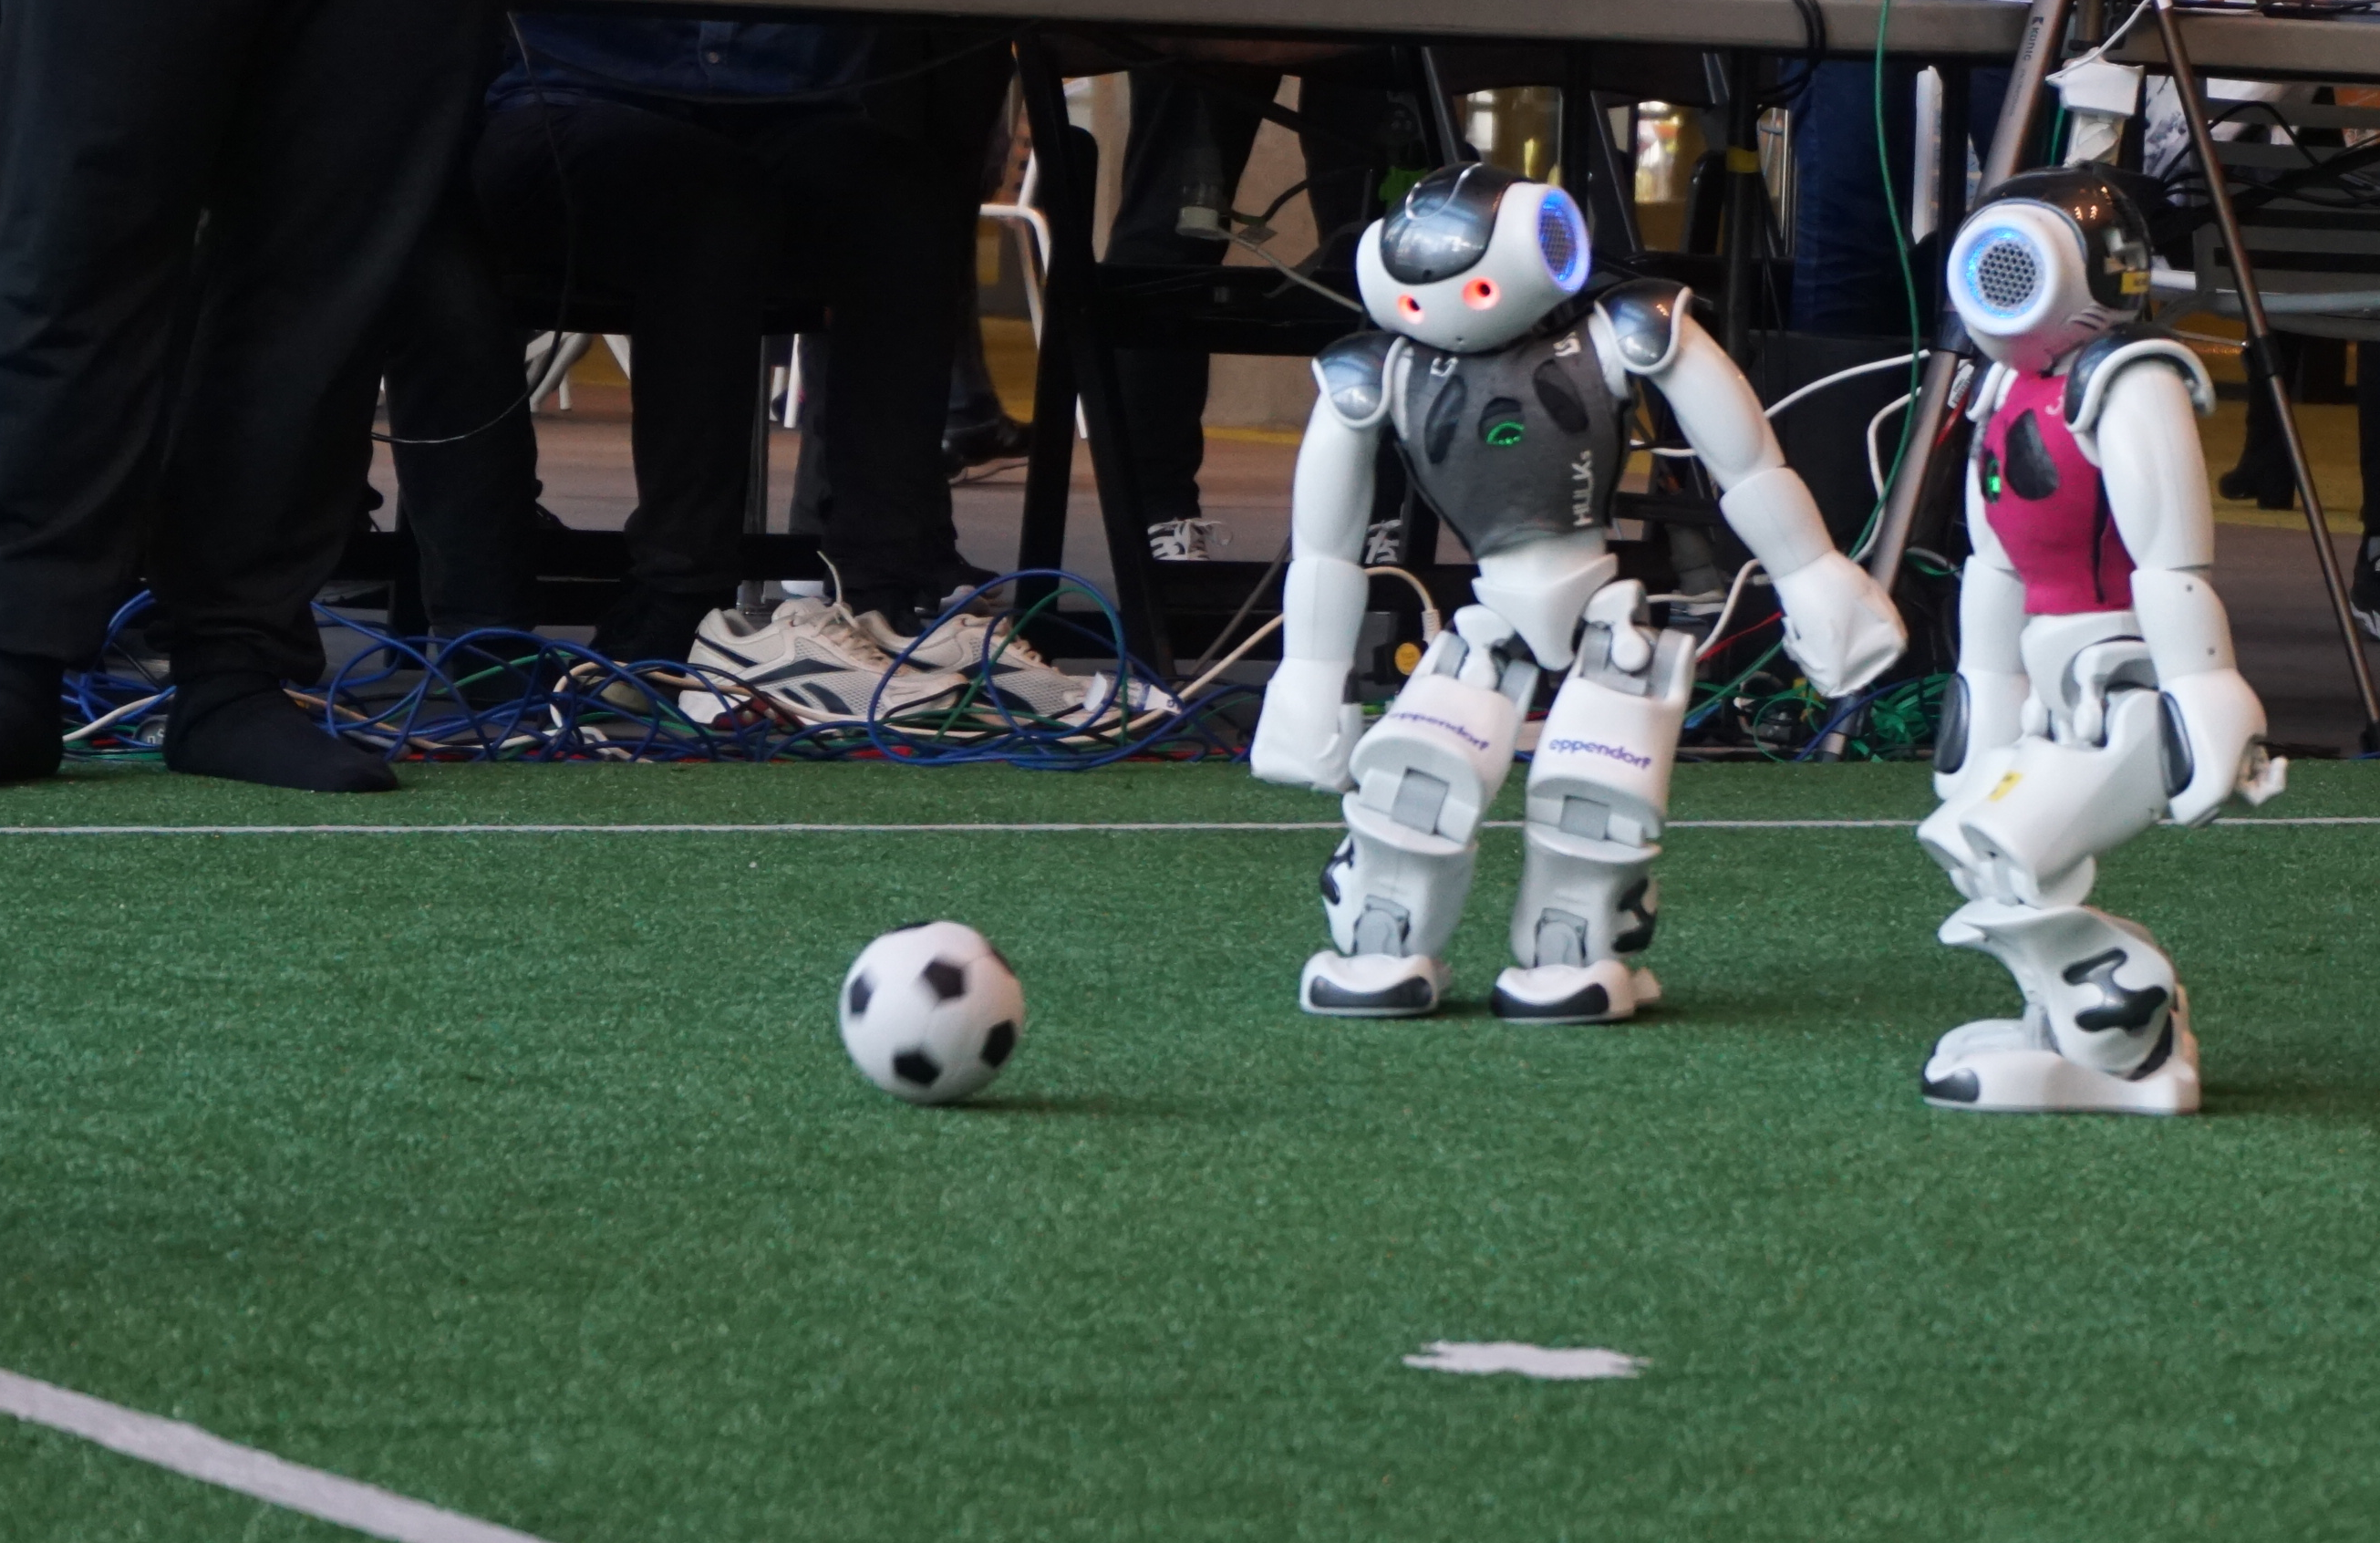
\includegraphics[width=0.6\columnwidth]{figures/robot}
	\caption[NAO robot]{V6 NAO robots while game play at the \ac{RoboCup} Sydney in 2019.}
	\label{fig:01_robot}
\end{figure}
% -------------------------------------------------------------

Within this scope, a \acf{WSL} competition \textit{Directional Whistle Challenge} was
introduced as technical challenge in 2019 that acted as initiator for this work.
The technical challenge covers smaller game independent tasks to test the realizability of
concepts and investigate preliminary ideas that might affect the prospective rules for the games.
By slightly changing the rules every year, the difficulty is increased and the conditions
are adapted to reach the level of human soccer as overarching goal until 2050.
Content of 2019's challenge specified to locate the position of a whistle blown by a referee
with one or multiple robots on the soccer field.
So far, whistles are only used for indicating the kick off of a game.
However, future consideration exist to use the whistle more frequent
to mark game state changes.
%  like executions of free kicks which include corner kicks or kick-ins.
Currently, the issue occurs that robots detect whistles of neighboring
games and start playing ahead of the own game start what yields to a penalty.
With increasing function of whistles, this difficulty propagates.

As another imaginable case of application, a \ac{SSL} can operate as confirmation
functionality between team members.
For example, the own keeper could send a audio output while an offensive player prepares
to shoot a goal.
If this audio signal is detected in the front by the offensive player, he recognizes
that he is about to score a own goal.
Potential mistakes and failure of other program components can be corrected by such
confirmation behavior between the robots.
For this reason, it was taken care that the implemented result is not limited to
whistle sounds.

\section{Objective}
\label{sec:01_objective}

For elaboration of this thesis, the sixth generation of NAO robots are being used
which consists of four microphones attached on the robot's head.
Detailed information about the robots hardware relevant for this work are presented
in \cref{subsec:03_microphones}.
For development on the NAOs, a extensive software framework is provided by the
\ac{SPL} team \textit{HULKs} which is student association at the \ac{TUHH}.
As a stable whistle detection exist already in this framework,
it will be utilized for the development of the \ac{SSL}.
Its high reliability stated in \cite{Hasselbring} was proven to be true at
competitions in the past.
False positives only occur when whistles are heard from other fields as explained above.

% Thus, SSL would be very helpful to prevent false starts
% To realise a SSL ->
% Use available whistle detection,
% This method implies that the utilized system must be attached with multiple microphones.
% make microphone channel available
% find appropriate method to localize on single robot
% Make multi-agent decision based on the wsde of the individual/stand-alone systems

% hulks software framework for whole set up and tests
% we have whistle detection, is very stable instead 

% say that all measurements were done in lab -> in evaluation part
% conclusion -> multimodales filtering, expizite ausreißerfilter, include prior knowledge
% of refree position
% evaluation -> SSD at beginning